\chapter{Grundlagen der Elektronenstoßionisation}
\label{chap:ion}
Das grundlegende Prinzip auf dem die Ionisation in einem RIT und die massenspektrometrische Messung dieser Arbeit basieren ist die Elektronenstoßionisation von Atomen, Molekülen und Ionen. 
Elektronenstoßionisation war bereits in den 1920er Jahren eine der ersten Methoden zur gezielten Ionisation von Teilchen für Massenspektrometrie und ist ein allgemein sehr relevanter Prozess, der Teil vieler Phänomene und Messmethoden in der Plasmaphysik ist. Beschrieben wird die Kollision eines extern beschleunigten Elektrons mit einem Atom, Molekül oder Ion in fester oder gasförmiger Phase. Im Folgenden werden die physikalischen Grundlagen dieses Prozesses erläutert. 

Bei der Kollision eines Elektrons mit einem Atom, Molekül oder Ion können im Wesentlichen die folgenden Mechanismen ausgelöst werden: elastische Streuung, Anregung und Ionisation. Bei Ionen ist es außerdem möglich, das diese mit dem Elektron rekombinieren. Welche dieser Mechanismen stattfinden hängt stark von der Energie des Elektrons ab und sie unterscheiden sich darin, wie viel Energie das Elektron an das Target überträgt. Der für diese Arbeit relevante Mechanismus ist die Ionisation. Folgende Abschnitte orientieren sich strukturell an der Arbeit von \cite{Ebinger}.

\section{Ionisationsprozesse}
Kommt es zur Ionisation können bei der Kollision $n$ gebundene Elektronen aus dem Target $A$ herausgelöst werden. $A$ trägt die Ladung $q$ (0 für neutrale Atome oder Moleküle) und es ensteht ein $(q+n)$-fach geladenes Ion. Folgende Reaktionsgleichung beschreibt die Stoßionisation eines Atoms im Allgemeinen.

\begin{equation}
     A^{q+} + e^- \rightarrow A^{(q+n)+} + (n + 1) e^-
\end{equation}

Von der Energie des stoßenden Elektrons hängt dabei ab, welche Prozesse auftreten können und wie viele Elektronen herausgelöst werden, dabei muss die Gleichung teilweise um Zwischenschritte erweitert werden. Das Elektron wird inelastisch im Coulombpotential des Atoms gestreut und gibt dabei Energie an ein im Atom gebundenes Elektron abgeben. Zum Herauslösen des gebundenen Elektrons muss die Energie des stoßenden Elektrons ausreichend groß sein und es ergibt sich eine charakteristische Ionisationsschwelle des Targets, bei der Ionisation überhaupt erst stattfinden kann. Die Ionisationsenergie $E_i$ ist dabei die Differenz aus den kinetischen Energien der freien Elektronen vor und nach dem Stoß: 
\begin{equation}
    E_i = E_{1,Kin, vor} - (E_{1,Kin, nach} + E_{2,Kin, nach}).
\end{equation} 
Wird ein gebundens Elektron durch den Energieübertrag direkt herausgelöst wird der Prozess als direkte Ionisation (engl. \textit{direct ionisation}, DI) bezeichnet. Direkte Ionisation ist fast immer der dominierende Vorgang bei Stoßionisation. Bei höheren Energien können allerdings auch indirekte, mehrstufige Prozesse auftreten, die auch zur Ionisation des Targets führen. Die erzeugten Ionen können allerdings im Nachhinein nicht unterschieden werden und tragen aber trotzdem einen Anteil am gesamten Ionisationsquerschnitt.

\subsection{Mehrstufige Ionisationsprozesse}
Der dominanteste mehrstufiger Prozess ist die Anregungs-Autoionisation (engl. \textit{exitation ionisation}, EA). Dabei wird ein auf einer niedrigen Schale gebundenes Elektron zunächst durch den Energieübertrag in einen höheren energetischen Zustand angeregt. Der daraus resultierende Zustand des Targets ist instabil und das Elektron fällt nach kurzer Zeit in den Grundzustand zurück. Dabei kann die Energie auch, anstelle einer Photon-Emission, an ein weiteres gebundenes Elektron in einer äußeren Schale weitergegeben werden, was für dessen Ausstoß aus dem Atom sorgt. Dieser Mechanismus ist als Auger-Prozess bekannt und stößt Elektronen nur mit einer für die Bindungszustände des Atoms charakteristischen Energie aus. Er ist in Abb. \ref{fig:EA} veranschaulicht.
\begin{figure}[h]
    \centering
    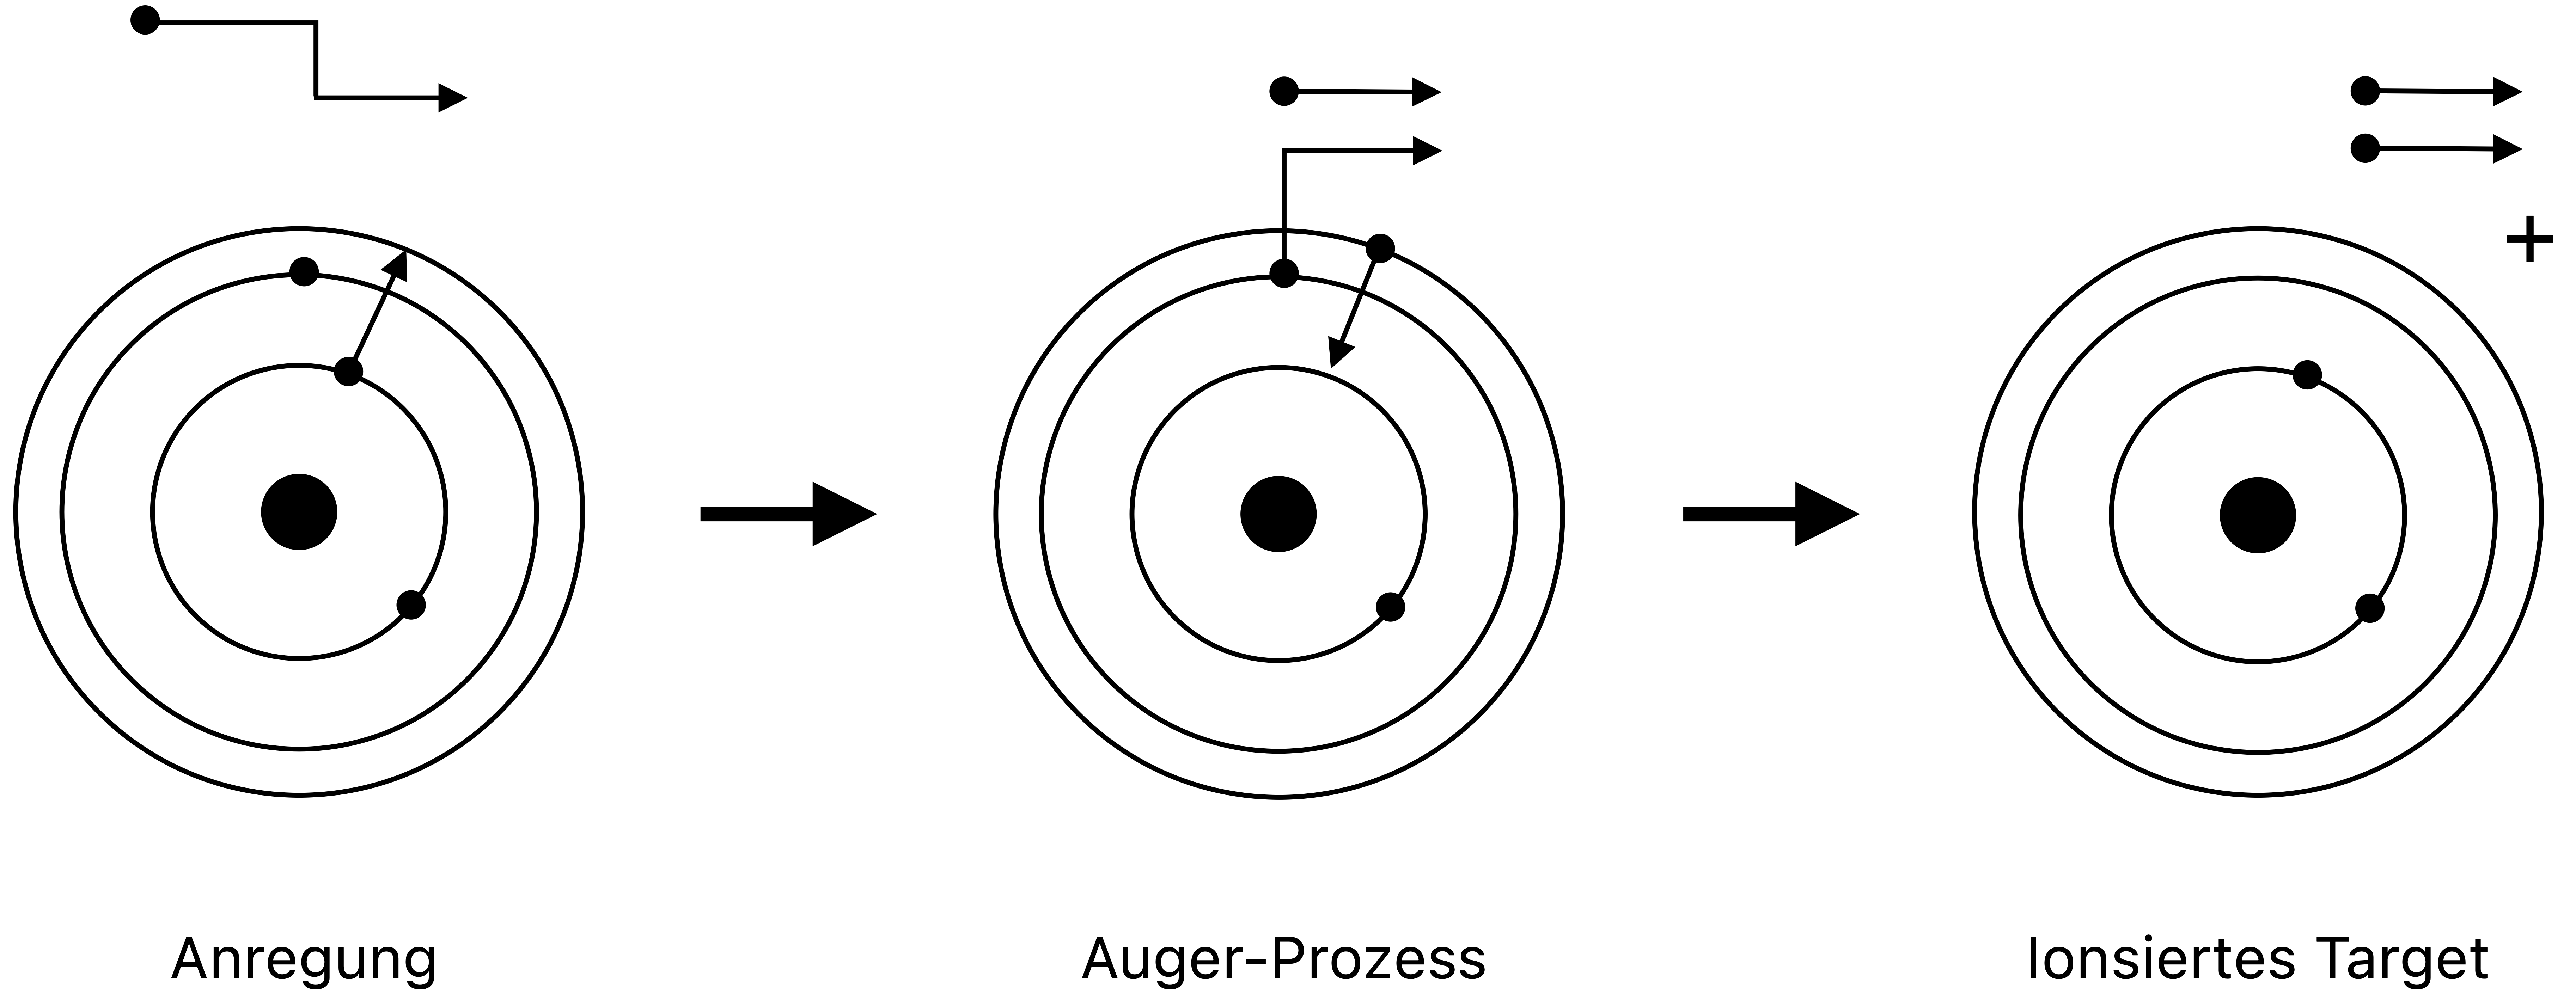
\includegraphics[width=.9\textwidth]{EA.png}
    \caption{Schematische Darstellung der Anregungs-Autoionisation für ein Atom.}
    \label{fig:EA}
\end{figure}
Weil bei der Anregungs-Autoionisation sowohl das Coloumb-Potential des Targets als auch die nötige Energie für die Anregung eines Elektrons überwunden werden müssen, tritt dieser Prozess erst bei höheren Energien auf. Bei Atomen mit gefüllten Schalen und wenigen Valenzelektronen (z.B. Alkaliatomen) können indirekte Prozesse eine große Rolle spielen, die auch der DI deutlich überlegen sein können \cite{EII}. Bei Argon ist der Anteil der EA allerdings gegenüber der DI fast vernachlässigbar klein. 

Es ist auch möglich eine Kombination aus DI und EA zu beobachten, bei der durch den Energieübertrag direkt ein Elektron aus einer inneren Schale herausgelöst wird und so das Target eine instabile Elektronenkonfiguration bekommt. Bei der folgenden Abregung kann es dann auch zum Auger-Prozess kommen. Mit steigender Energie des stoßenden Elektrons steigt die Wahrscheinlichkeit für mehrstufige Prozesse und es sind noch höhere Anregungen, die zu Mehrfachionisationen über Auger-Kaskaden führen, möglich.

Bei Molekülen kann es dazu kommen, dass das aus der Wechselwirkung resultierende ionisierte Molekül nicht stabil ist und es zur Dissoziation kommt oder das Molekül vom Stoß eines Elektrons mit hoher Energie direkt dissoziiert wird. Dabei werden häufig Ionen oder Radikale gebildet, es können aber auch neutrale Fragmente entstehen. Dieser Vorgang wird als Dissoziationsionisation (engl. \textit{dissociative ionisation}, auch DI aber im Folgenden als DIS) bezeichnet, wenn der Zerfall aufgrund von Ionisation stattfindet. Ein solcher Prozess kann durch eine der folgende Reaktionsgleichungen beschrieben werden:
\begin{equation}
    AB + e^- \rightarrow A^{+} + B + 2e^-
\end{equation}
\begin{equation}
    AB + e^- \rightarrow AB^* + e^- \rightarrow A^{+} + B + 2e^-.
\end{equation} 
Hierbei ist $AB$ das Molekül und $AB^*$ das angeregte Molekül.

Über eine Reihe von Stoßionisationen können komplexe Moleküle so in viele verschiedene, kleinere Fragmente zerfallen. Aufgrund dieser hohen Fragmentierung wird die Elektronenstoßionisation als eine \textit{harte} Ionisationsmethode bezeichnet.

\subsection{Resonante Prozesse}
Bei der Ionisation von Atomen und Molekülen kann auch ein resonanter Prozess einen Zwischenschritt darstellen. Dabei wird das Elektron vom Target \textit{eingefangen} und verbleibt nicht im Kontinuum (freien Zustand). Man spricht von Resonanz, da die Energie des Elektrons genau einem quantiesierten Energieniveau im Atom entsprechen muss, um temporär gebunden zu werden. Mit derselben Argumentation könnten auch die EA-Prozesse als resonant bezeichnet werden, da sie den gleichen diskreten Energieniveaus unterliegen. Als resonante Prozesse werden dennoch üblicherweise nur die bezeichnet, die mit dem einfallenden Elektron verbunden sind.

Der bei einem solchen resonanten Prozess entstehende Energiezustand kann allerdings nicht wirklich als Energieniveau bezeichnet werden, da er über der Ionisationsenergie liegt \cite{EII}. Der Zustand ist instabil und endet häufig in Autoionisation. Da Moleküle aufgrund ihrer zusätzlichen Freiheitsgrade (Rotation, Schwingung) und überlappenden Orbitalen mehr diskrete Energieniveaus haben, sind resonante Prozesse beim Stoß von Elektronen mit Molekülen häufiger. Das sorgt auch für zusätzliche Dissoziation und wird als dissioziative Elektronenanlagerung (engl. \textit{Dissociative Electron Attachment}, DEA) bezeichnet, wenn dieses beim Einfang des Elektrons zerfällt. Resonante Ionisationsprozesse treten zudem besonders beim Stoß von Elektronen und Ionen auf, weil das positive Potential anziehend auf das Elektron wirkt und haben somit weniger Relevanz bei der Ionisation von Atomen.

\section{Ionisierungsquerschnitt}
Der Ionisierungsquerschnitt beschreibt, wie effektiv das Analytgas ionisiert werden kann. Der Querschnitt setzt sich dabei aus den einzelnen Querschnitten der verschiedenen, beschriebenen Ionisationsprozesse zusammen, kann aber in dem in dieser Arbeit beschriebenen Experiment nur integral aufgenommen werden. Er kann allerdings für jede der verschiedenen Ionenarten aufgenommen und die Anteile ermittelt werden. Aus der Summe aller ionischen Produkte ergibt sich ein Gesamtionisierungsquerschnitt. Unter der Bedingung, dass nur sehr wenige der Elektronen eine Kollision mit einem Targetatom haben, kann der Stoßionisierungsquerschnitt wie folgt beschrieben werden:

\begin{equation}
    \sigma_{\text{i}}(A^{q+}) = \frac{N_{\text{i}}(A^{q+})}{N_{\text{e}} \cdot n l}.
\end{equation}

$N_i(A^{q+})$ ist dabei die Anzahl der erzeugten Ionen $A^{q+}$ und $N_e$ die Anzahl der Elektronen. $n$ ist die Teilchendichte des Gases und $l$ die Länge der Strecke, die die Elektronen im Gas zurücklegen. Einfach hergeleitet werden kann diese Formel über die Wahrscheinlichkeit $P(A^{q+})$, die ein Elektron besitzt die gesuchte Ionisation durchzuführen. Diese ist gleich dem Verhältnis der Anzahl der Stoßionisationen die zum gesuchten Ion führen zur Anzahl der Elektronen, wie auch dem Produkt aus der Teilchendichte, der zurückgelegten Strecke und dem Stoßionisierungsquerschnitt: 
\begin{equation}
    P(A^{q+}) = \frac{N_{\text{i}}(A^{q+})}{N_e} = n \cdot l \cdot \sigma_i(A^{q+}).
\end{equation}
Da später nur ein Teil der erzeugten Ionen von einem Detektor nachgewiesen werden kann, wird für $l$ nur der auf der aktiven Fläche des Detektors sichtbare Teil des Elektronenstrahls verwendet. Aus diesem kann die für das Experiment effektive Länge $l$ abgeleitet werden.

Wie leicht zu erkennen ist, ist die genaue Messung der Elektronen- und Ionenzahlen für eine akkurate Aufnahme der Ionisierungsquerschnitte zentral. Außerdem wird angenommen, dass die Einzelstoßbedingung erfüllt ist. Diese wird in \ref{chap:Einzelstoß} erläutert. Um eine absolute Aussage treffen zu können, muss auch die Teilchendichte des Gases absolut bestimmt werden.


\section{Ansätze theoretischer Beschreibungen}
Die theoretische Beschreibung von Elektronenstoßionisation ist ein hochkomplexes Problem. Selbst bei der einfachen DI gibt es im finalen Zustand drei freien Teilchen, die über die Coulombkraft miteinander wechselwirken. Dabei handelt es sich um das famose Drei-Körper-Problem, für das es keine analytische Lösung gibt. Für die Wechselwirkung mit den gebundenen Zuständen im Atom wird eine quantenmechanische Beschreibung vom Atom gefordert. Während mit der Schrödingergleichung und numerischen Methoden inzwischen Atome mit vielen gebundenen Zuständen gut approximiert werden können, wird die Beschreibung des Problems mit gebundenen und mehreren freien Elektronen sehr schnell sehr komplex. Trotzdem sind einige Ansätze entwickelt worden, die die Stoßionisierungsquerschnitte für Atome gut nähern können.

\subsection{Lotz-Formel}
Eine empirische Formel zur Berechnung des Ionisationsquerschnitts entwickelte Wolfgang Lotz Ende der 1960er Jahre \cite{Lotz}. Mit dieser kann eine praktische Abschätzung des Ionisierungsquerschnitts gemacht werden. Die Formel basiert auf experimentellen Daten und berücksichtigt nur die direkte Ionisation. Trotzdem liefert sie gute Näherungen für die Ionisation von Atomen bei geringeren Elektronenenergien und ist auch für die Bestimmung der Ionisationsschwelle geeignet. Die Lotz-Formel ist gegeben durch den Ausdruck:
\begin{equation}
    \sigma = \sum_{i=1}^{N} a_i n_i \frac{ \ln (E_e / P_i) }{E_e P_i} \left( 1 - b_i e ^{-c_i (E_e / P_i-1)}\right).
\end{equation}
Dabei sind $a_i$, $b_i$ und $c_i$ Konstanten, die für jedes Target spezifisch sind. $E_e$ ist die Energie des einfallenden Elektrons. Die Lotz-Formel nimmt an, dass alle $n_i$ Elektronen jeder Schale einen Beitrag zum Gesamtionisationsquerschnitt machen können, solange ihre Bindungsenergie $P_i$ kleiner als $E_e$ ist. Daher wird über die $N$ Schalen des Targets eine Summe gebildet. Die Formel kann auch für Moleküle verwendet werden, wenn die Ionisationsenergien bekannt sind.

\subsection{Störungstheorie}
Die Idee der Störungstheorie ist es, ein komplexes quantenmechanisches Problem, das analytisch nicht lösbar ist, aber einem lösbareren Problem ähnelt, als das lösbare Problem plus eine Störung zu betrachten. Hierbei wird der Hamiltonoperator $\hat{\mathcal{H}}$ in einen Teil für das ungestörte Atom und einen Störterm $\hat{\mathcal{V}}$ aufgeteilt:
\begin{equation}
    \hat{\mathcal{H}} = \hat{\mathcal{H}}_{Atom} + \hat{\mathcal{V}}.
\end{equation}
Dieser wird dann zur Lösung der Schrödingergleichung verwendet, wobei $\Psi$ die Wellenfunktion des Systems ist:
\begin{equation}
    \hat{\mathcal{H}} \Psi = i\hslash\frac{\partial}{\partial t}\Psi.
\end{equation}
Wie der Störterm gewählt wird, hängt vom gewählten Ansatz ab und ist entscheidend für die Komplexität und Genauigkeit der Rechnung. Um die Stoßionisation zu beschreiben, muss der Störterm so gewählt werden, dass er die Wechselwirkung zwischen dem einfallenden Elektron und dem Atom beschreibt. Dafür werden verschiedene vereinfachte Modelle verwendet, die je nur unter bestimmten Bedingungen gute Näherungen der Ionisationsquerschnitte liefern. Eine unnachgiebige Lösung wurde noch nicht gefunden, besonders wenn versucht wird die Ionisation von Molekülen oder indirekte Prozesse zu beschreiben. Die meisten Ansätze haben gemeinsam, dass $\hat{\mathcal{V}} = \hat{\mathcal{V}}_{e^-} + \hat{\mathcal{V}}_{WW}$ wählen, wobei $\hat{\mathcal{V}}_{e^-}$ das Elektron und $\hat{\mathcal{V}}_{WW}$ die Wechselwirkung  beschreibt. 

Die folgende Beschreibung orientiert sich an der von Younger \cite{EII}. Einige Methoden basieren auf der Partialwellen-Approximation (engl. \textit{Partial Wave Approximation}, PWA), bei der die Wellenfunktion $\Psi$ jedes Elektrons als eine Kugelwelle beschrieben wird. Die Gesamtwellenfunktion ist dann die Summe der einzelnen Kugelwellen:
\begin{equation}
    \Psi (\vec K, \vec r) = \sum_{lm}a_{lm}Y_{lm}(\theta, \phi) F_l(K,r).
\end{equation}
Dabei sind $Y_{lm}(\theta,\phi)$ die winkelabhängigen Kugelflächenfunktionen und $F_l(K,r)$ die Radialfunktionen, die vom Abstand $r$ abhängt und bei der $K$ den Impuls des Elektrons beschreibt. $a_{lm}$ ist die Amplitude der Kugelwelle. $F_l(K,r)$ muss die radiale Schrödingergleichung erfüllen. Bei einem kugelsymmetrischen Potential ist die radialen Schrödingergleichung
\begin{equation}
    E u = \underbrace{\frac{\hslash^2}{2m}\frac{d^2 u}{dr^2}}_{\substack{\text{$E_{Kin}$-Term}}} + \left[\underbrace{\frac{\hslash^2}{2m} \frac{l(l+1)}{r^2}}_{\substack{\text{Zentrifugalterm}}} + \underbrace{V(r)}_{\substack{\text{Potential}}} \right] u.
\end{equation}
Dabei wird $u(K,r) = rF_l(K,r)$ verwendet, um die Rechnung zu vereinfachen.
Wenn die Interaktion in der Nähe des Atomkerns beschrieben werden soll ($Kr \ll 1$), kann keiner der Terme vernachlässigt werden. Verschiedene Ansätze unterscheiden sich in der Wahl des Potentials $V(r)$. 

Bei der Plane-Wave Born Approximation wird das Potential als $V(r) = 0$ angenommen, was nur für sehr hohe Elektronenenergien gute Näherungen liefert und der Beschreibung reiner Elektronenstreuung ähnelt.

Eine andere Wahl ist $V(r) = -\frac{Z}{r}$, was dem Coulombpotential des Atomkerns entspricht. Dieser Ansatz wird als Coulomb-Approximation bezeichnet und eignet sich zur Beschreibung der Ionisation von Ionen.

Die Distorted-Wave Born Approximation fügt dem Potential noch einen Störterm hinzu, der die gebundenen Elektronen beschreiben soll. Dieser Ansatz ist für die Beschreibung der Ionisation von Atomen besser geeignet, da er die Wechselwirkung zwischen dem einfallenden Elektron und den gebundenen Elektronen besser beschreibt. Der Rechenaufwand ist allerdings schnell sehr hoch.

Neben störungstheoretischen Ansätzen gibt es auch andere Methoden, die mit größerem Aufwand bessere Näherungen liefern. Dazu gehören rein numerische Methoden und hybride Ansätze, die störungstheoretische und numerische Methoden kombinieren. Da in dieser Arbeit keine theoretische Beschreibung der Ionisation durchgeführt wird, wird hier nicht weiter auf die Methoden eingegangen.

Zusammenfassend kann gesagt werden, dass die theoretische Beschreibung der Elektronenstoßionisation noch teil aktueller Forschung ist und in der Realität häufig auf empirische Daten zurückgegriffen weden muss, um Ergebnisse zu vergleichen. Im Rahmen dieser Arbeit wird Straubs Arbeit \cite{Straub} mehrfach als Referenz verwendendet. 

\section{Einzelstoßbedingung}
\label{chap:Einzelstoß}
Unter dem Begriff Einzelstoßbedingung werden zwei unterschiedliche, für diese Arbeit relevante Aspekte beschrieben: die Anzahl der Wechselwirkungspartner aus der Perspektive eines Atoms und die Anzahl der Stöße beim Durchqueren des Gases aus der Perspektive eines Elektrons. Sie werden im Folgenden getrennt betrachtet und erläutert.

\subsection{Einzelstoßbedingung aus der Perspektive des Atoms}
Alle der soeben genannten Prozesse, sowie Beschreibungen wurden unter der Annahme erläutert, dass nur ein einzelnes Elektron gleichtzeitg mit einem Target im einfallenden Zustand wechselwirkt. Diese Annahme dient dazu, die Ionisationsprozesse in ihrer einfachsten Form betrachten und analysieren zu können, ohne noch komplexere Mehrteilchenprozesse berücksichtigen zu müssen. Die Interaktion findet dann unter der Einzelstoßbedingung statt. Auch wenn die Einzelstoßbedingung in einem RIT in der Regel nicht erfüllt ist, ist sie für die Messung des Ionisierungsquerschnitts in dieser Arbeit essenziell. Denn nur so kann die Anzahl der erzeugten Ionen mit der Anzahl der Elektronen sinnvoll in Beziehung gesetzt werden und mit dem Lotz-Plott verglichen werden. Ob diese Einzelstoßbedingung erfüllt ist, hängt im Wesentlichen von der Elektronendichte ab. Diese kann über den Extraktionsstrom der Elektronenkanone und die Strahlzeit eingestellt werden.

Außerdem ist zu beachten, dass mehrere Wechselwirkungen, die nacheinander jeweils nur mit einem Elektron stattfinden, auch zur Verfälschung der Messung führen können. Ein Atom kann über mehrere einfache DI-Prozesse mehrfach ionisiert werden und das Ion kann im Nachhinein nicht von einem mehrfach geladenen Ion unterschieden werden, das durch einen einzelnen Prozess entstanden ist. Insofern kann auch hier die Einzelstoßbedingung verletzt sein. In dieser Arbeit kann dieser Effekt vermieden werden, in dem die Strahlzeiten der Elektronenkanone so kurz gewählt werden, dass die Wahrscheinlichkeit für mehrfache Ionisationen sehr gering ist.

\subsection{Einzelstoßbedingung aus der Perspektive des Elektrons}
Betrachtet man ein Elektron, was ein Gas durchquert, so hängt die Anzahl der Stöße mit Atomen aus diesem Gas von der mittleren freien Weglänge $\lambda$ und der durch das Gas zurückgelegten Entfernung $d$ ab. Die mittlere freie Weglänge ist dabei die durchschnittliche Entfernung, die ein Elektron zurücklegt, bevor es mit einem Atom wechselwirkt und ist gegeben durch:
\begin{equation}
    \lambda = \frac{1}{n \cdot \sigma},
\end{equation}
wobei $n$ die Teilchendichte und $\sigma$ der Stoßquerschnitt ist.
Folgende Beziehung beschreibt die mittlere Anzahl der Stöße $N$:
\begin{equation}
    N = \frac{d}{\lambda}.
\end{equation}
Wenn man eine rein klassische Abschätzung macht und die Atome als harte Kugeln annimmt, kann der Wirkungsquerschnitt als eine Fläche mit dem Radius des Atoms beschrieben werden. Wichtig ist, das $N$ deutlich kleiner als 1 ist, um die Einzelstoßbedingung für jedes Elektron zu erfüllen. 